\chapter{RESULTS AND DISCUSSION}
\section{Steady States and their Stability}
\subsection{Equilibrium Points}
The points of equilibrium are achieved using the following set of equations and
 dynamics of the model is analyzed using these set of points:
\begin{equation}\frac{d S_1}{dt} = 0 = \frac{d I_1}{dt}=\frac{d Q_1}{dt}=\frac{d R_1}{dt}=\frac{d I_2}{dt}=\frac{d B_2}{dt}=\frac{d R_2}{dt}\end{equation}
from the system of targeted and attacker class equations.
If infection is not present in the system, then it has following malicious codes-free equilibrium state:
\begin{equation*}E_1 = (1, 0, 0, 0, \hat I_2, \hat B_2,\hat R_2),\end{equation*}
and one endemic equilibrium state:
\begin{equation*}E_2 = (\check S_1,\check I_1 ,\check Q_1,\check R_1,\check I_2, \check B_2,\check R_2 ).\end{equation*}
Here it is retrieved that the equilibrium point $E_1$ is on the $S_1$ - $I_2$ - $B_2$ - $R_2$ plane and is always possible since all the other parameters are greater than 0.
For the calculation of the feasibility of
 the endemic steady state $E_2$ for different parameter sets, the numerical values of parameters are adopted.
The expressions for the equilibrium points are used to retrieve the conditions for
 stability of malicious-code free solutions. To avoid infection propagation, it will be advantageous
to get the minimum recovery rate.
\clearpage
\section{Basic Reproduction Number}
The anticipated number of secondary infection cases
 originated by a single infection in an entirely susceptible population is called Basic reproduction number, $R_0$. To
 characterize the malicious object propagation, it is considered as one of the most useful
 barrier (threshold parameter) \cite{edtr18}.
Let
\begin{equation*} x= ( I_1, Q_1, I_2, B_2 ).\end{equation*}
 Then, the derivative of infection classes, i.e., equations (2.13)
 and (2.14) of targeted system and equations (2.16)
 and (2.17) equations of attacker system is given by,
\begin{equation}\frac{d x}{d t} =\mathcal F -\mathcal V,\end{equation}
Where,
\[
\mathcal F=
\begin{bmatrix}
\beta_1 e^{-m_1 I_1} I_1 S_1- \beta_2 e^{-m_2 B_2} B_2 N_2 S_1 \\
Q_1 S_1 \\
0 \\
0
\end{bmatrix},
\]
\[
\mathcal V=
\begin{bmatrix}
( d_2+ \eta + \mu) I_1+ \frac{ I_1}{N_1}-d_2 I_1^2- I_1 S_1-d_2 Q_1 I_1-I_1 R_1\\
- \mu I_1 + d_2 Q_1 + \lambda_0 Q_1+ \frac{ Q_1}{N_1}-d_2 Q_1^2-d_2 I_1 Q_1-Q_1 R_1\\
- \frac{( 1- I_2)}{N_2}+ d_4 I_2+\delta I_2 - \theta R_2 +\eta_1 I_2- d_4 I_2^2-d_4 I_2 B_2- I_2 R_2\\
-\delta I_2 + d_4 B_2 +\gamma B_2+ \frac{ B_2}{N_2}-d_4 B_2^2-d_4 I_2 B_2- B_2 R_2
\end{bmatrix},
\]
Therefore,\\
F(Jacobian of F at malicious codes-free equilibrium)=
\[
\begin{bmatrix}
(\beta_1+1) S_1 & 0 & 0 & \beta_2 S_1 \\
0 & S_1 & 0 & 0 \\
0 & 0 & 0 & 0 \\
0 & 0 & 0 & 0
\end{bmatrix},
\]
and,\\
V(Jacobian of V at malicious codes-free equilibrium)=
\[
\begin{bmatrix}
( d_2+ \eta + \mu+1) & 0 & 0 & 0 \\
-\mu & (d_2+\lambda_0+1) & 0 & 0 \\
0 & 0 & (1+d_4+\delta+\eta_1) & 0 \\
0 & 0 & -\delta & (d_4+\gamma+1)
\end{bmatrix}.
\]
\par F is the rate matrix describing secondary infection, and V is the rate matrix
of the transmission. Then, the dominant eigenvalue of FV\textsuperscript{-1}
is called the basic reproduction number $R_{0}$ .
\begin{equation} R_0 = max \left\{\frac{(\beta_1+1) S_1}{(d_2+\mu+\eta+1)},\frac{S_1}{(d_2+\lambda_0+1)} \right\} , \end{equation}
\par Where $S_1$ shows the node density of susceptible nodes of targeted
 population in non endemic equilibrium state. This model has one such
 state $E_1$ and hence there is only one basic reproduction number $R_0$. Value of $R_0$ is:
For equilibrium state $E_1$,
$S_1$=1 and hence,
\begin{equation} R_0 = max \left\{\frac{(\beta_1+1)}{(d_2+\mu+\eta+1)},\frac{1}{(d_2+\lambda_0+1)} \right\} . \end{equation}
Applying the same procedure for the proposed system (2.4)-(2.10), we get basic reproduction number,
\begin{equation}\tilde R_0 =\frac{\tilde \beta_1}{(\tilde d_2+ \tilde \mu+\tilde \eta)} . \end{equation}

\section{ Local Asymptotic Stability}
The local asymptotic stability of both, malicious codes-free and endemic equilibrium, is
 specified. The generalized Jacobian matrix is given as follows:

\[
J=
\begin{bmatrix}
-2+2 S_1&d_2 S_1-\beta_1 S_1&d_2 S_1&\alpha+S_1&0&-\beta_2 S_1&0\\
0&a_{22}&0&0&0&\beta_2 S_1&0\\
0&\mu&a_{33}&0&0&0&0\\
0&\eta&\lambda_0&a_{44}&0&0&0\\
0&0&0&0&a_{55}&0&\theta\\
0&0&0&0&\delta&-1-d_4-\gamma&0\\
0&0&0&0&\eta_1&\gamma&-2-\theta\\
\end{bmatrix},
\]
Where,
\begin{eqnarray*}
a_{22}&=&-1-d_2-\eta-\mu+\beta_1 S_1+S_1, \\
a_{33}&=&-1-d_2-\lambda_0+S_1, \\
a_{44}&=&-2+\alpha+S_1,\\
a_{55}&=&-1-d_4-\eta_1-\delta.
\end{eqnarray*}
\clearpage
At non endemic equilibrium, the variation matrix $E$ is given below:
\[
J=
\begin{bmatrix}
0&d_2-\beta_1&d_2&1+\alpha&0&-\beta_2&0\\
0&\beta_1-d_2-\eta-\mu&0&0&0&\beta_2&0\\
0&\mu&-d_2-\lambda_0&0&0&0&0\\
0&\eta&\lambda_0&-1-\alpha&0&0&0\\
0&0&0&0&-1-d_4-\eta_1-\delta&0&\theta\\
0&0&0&0&\delta&-1-d_4-\gamma&0\\
0&0&0&0&\eta_1&\gamma&-2-\theta
\end{bmatrix}
\]
The eigenvalues of this matrix are:\{0, \hspace{0.5 cm}$ \beta_1-d_2-\eta-\mu, \hspace{0.5 cm} -d_2-\lambda_0, \hspace{0.5 cm} -1-\alpha$,\\
$\frac{ -(-2 a^3 + 3^{3/2} {(-4 a^3 d - a^2 c^2 + 18 a c d + 4 c^3 + 27 d^2)}^{1/2} + 9 a c + 27 d)^{1/3}}{(3*2^{1/3}) }$+\\ $\frac{(2^{1/3} (3 c - a^2))}{(3 (-2 a^3 + 3^{3/2} {(-4 a^3 d - a^2 c^2 + 18 a c d + 4 c^3 + 27 d^2)}^{1/2} + 9 a c + 27 d)^{1/3})}$ + $\frac{a}{3}$,\\
  $\frac{((1 - 3^{1/2} i){ (-2 a^3 + 3^{3/2} {(-4 a^3 d - a^2 c^2 + 18 a c d + 4 c^3 + 27 d^2)}^{1/2} + 9 a c + 27 d)}^{1/3})}{(6* 2^{1/3})}$\\ -$\frac {((1 +3^{1/2} i ) (3 c - a^2))}{{(3* 2^{2/3} (-2 a^3 + 3^{3/2} {(-4 a^3 d - a^2 c^2 + 18 a c d + 4 c^3 + 27 d^2}^{1/2} + 9 a c + 27 d}^{1/3}} $+$\frac{ a}{3}$,\\
  $\frac{((1 + 3^{1/2} i){ (-2 a^3 + 3^{3/2} {(-4 a^3 d - a^2 c^2 + 18 a c d + 4 c^3 + 27 d^2)}^{1/2} + 9 a c + 27 d)}^{1/3})}{(6* 2^{1/3})}$\\ -$\frac {((1 -3^{1/2} i ) (3 c - a^2))}{{(3 *2^{2/3} (-2 a^3 + 3^{3/2} {(-4 a^3 d - a^2 c^2 + 18 a c d + 4 c^3 + 27 d^2}^{1/2} + 9 a c + 27 d}^{1/3}} $+$\frac{ a}{3}$
\}.
Where,
\begin{eqnarray*}
a&=&-4-2 d_4-\eta_1-\delta-\gamma-\theta, \\
b&=&-1-b_4,\\
c&=&b^2-\gamma b- 2\theta b-4 b-\eta_1 b+\eta_1 \gamma+2\eta_1 \theta+2\eta_1-\delta b+\delta \gamma+\delta \theta+2\delta+2 \gamma+\theta\gamma, \\
d&=&\theta \eta_1 b+2 b^2-2\gamma b-2\eta_1 b+2\gamma\eta_1-2\delta b+2\delta\gamma+\theta b^2+\gamma\theta b-\delta \theta b.
\end{eqnarray*}
\par Equilibrium state $E_1$ is said to be locally asymptotically stable when all eigenvalues of $J_{01}$
variation matrix will be having negative real parts
 or when it is negative in nature. So, if $R_0$\textless1, then all the eigenvalues will possess negative real parts.
Hence, it can be said the malicious code free equilibrium $E_1$ is locally asymptotically unstable if $R_0$$>$1 and stable,
 if $R_0$\textless1.

\section{Numerical Experimentation}
Numerical methods are used to determine and analyze the system of equations for the targeted and attacker system. The behaviors of the nodes are examined for the different classes. The targeted and attacker system has been determined and simulated and the nature of the nodes in both of the classes are observed. All of these analyses are done concerning the time.
\subsection{Feasible Steady States}
In this step, possible steady states are simulated and analyzed for different parameter sets for the proposed model.
If all the classes possess non-negative values at any point, then a steady state is said to be feasible at that point. Table 3.1 shows the feasibility of steady states
related to the particular basic reproduction number and for different parameter set.
\par
Various curves are plotted to observe the nature of the classes with respect to time. These Graphical plots show
the density $S_1$, $I_1$, $Q_1$ and $R_1$ nodes of attacker class and $I_2$, $B_2$ and $R_2$ targeted class. Since $E_1$ is the malicious code free state so it would be present in all of the set of equilibrium states if their reproduction number $R_0$ \textless 1, otherwise equilibrium will tend to $E_2$
state if their $R_0$$>$1. All observations are done with respect to the time and with different parameter sets.
\begin{table}[h]

\label{table:feas}
\begin{tabular}{|p{3.5 cm}|l|l|p{3.5 cm}|l|l|}
\hline
\bf Parameters (Non-Dimensional) & \bf Set A& \bf Set B& \bf Parameters (With Dimensions)& \bf Set C& \bf Set D \\
\hline
b &7.5&7.5&b&1&75\\
$d_1$ &0.003&0.003&$d_1$&0.3&0.3\\
$\beta_1$ &0.001&0.01&$\tilde \beta_1$&0.5&2.5\\
$\beta_2$ &0.006&0.30&$\tilde\beta_2$&0.6&0.6\\
$\mu$ &0.003&0.003&$\tilde\mu$ &0.3&0.3\\
$\lambda_0$ &0.008&0.0008&$\tilde\lambda_0$&0.8&0.8\\
$d_4$ &0.075&0.0075&$\tilde d_4$&10&2.5\\
$b_1$ &7.5&7.5&$\tilde b_1$ &75&75\\
$d_3$ &0.02&0.02&$\tilde d_3$&2.0&2.0\\
$\eta$ &0.004&0.0004&$\tilde\eta$ &0.4&0.4\\
$\eta_1$ &0.175&0.0175&$\tilde\eta_1$&17.5&7.5\\
$\alpha$ &0.010&0.0005&$\tilde\alpha$&1.0&1.0\\
$d_2$ &0.4&0.004&$\tilde d_2$&0.4&0.4\\
$\gamma$ &0.0005&0.01&$\tilde\gamma$ &0.75&0.75\\
$\delta$&0.009&0.027&$\tilde\delta$&1.9&0.9\\
$\theta$ &0.10&0.20&$\tilde\theta$&10&10\\
$m_1$ &2&2&$m_1$&6&2\\
$m_2$ &3&2&$m_2$&6&2\\
\hline
Feasible SS&$E_1$&$E_2$&Feasible SS&$E_1$&$E_2$\\
\hline
$R_{01}$&0.0098&1.2500&&&\\
$R_{02}$&0.0073&0.3846&$\tilde R_{0}$&0.4545&2.2727\\
\hline
\end{tabular}
\caption {Possible steady states with respect to the reproduction number for different parameter
set(Dimensional and non-dimensional) in the model }
\end{table}
\begin{figure}
\centerline{\includegraphics[width=15cm,height=10cm]{13-DR2}}
\caption{Graph between node density and time for set A with initial population (0.4, 0.02, 0.02, 0.2, 0.50, 0.25, 0.25)}
\label{fig:13-DR2}
\end{figure}
\begin{figure}
\centerline{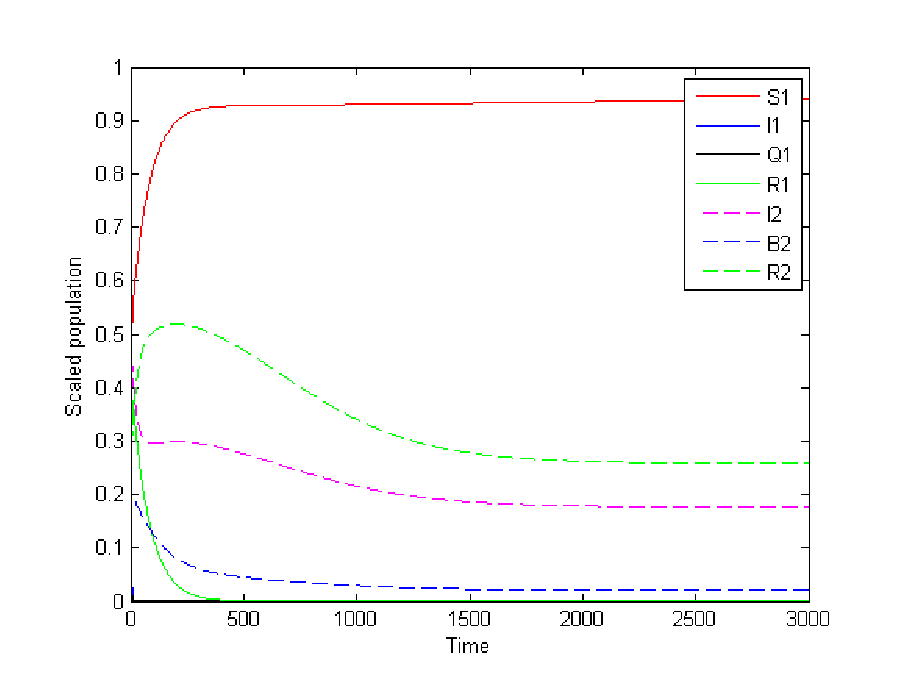
\includegraphics[width=15cm,height=10cm]{13-DR3}}
\caption{Graph between node density and time for set A with initial population (0.30, 0.30, 0.11, 0.25, 0.50, 0.20, 0.25)}
\label{fig:13-DR3}
\end{figure}
\begin{figure}
\centerline{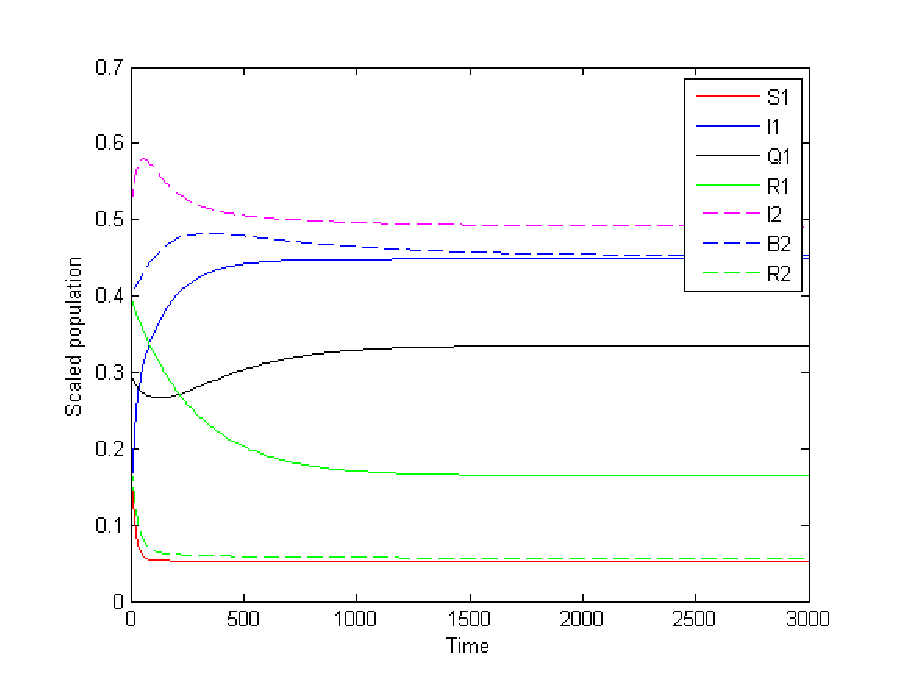
\includegraphics[width=15cm,height=10cm]{13-DR4}}
\caption{Graph between node density and time for set B with initial population (0.2, 0.1, 0.3, 0.4, 0.5, 0.4, 0.2)}
\label{fig:13-DR4}
\end{figure}
\begin{figure}
\centerline{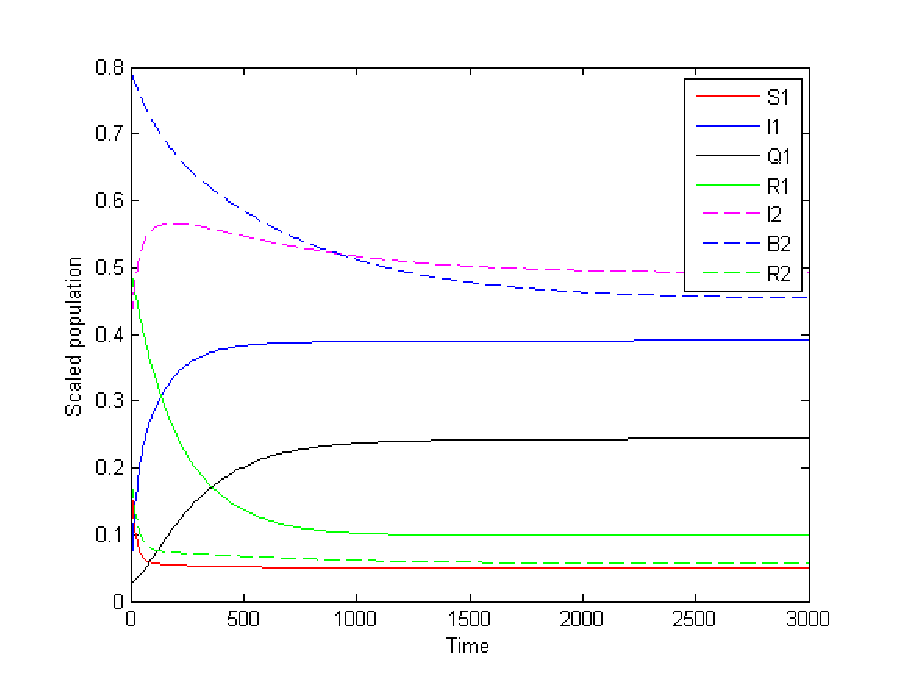
\includegraphics[width=15cm,height=10cm]{13-DR8}}
\caption{Graph between node density and time for set B with initial population (0.2, 0.01, 0.03, 0.5, 0.4, 0.8, 0.2)}
\label{fig:13-DR8}
\end{figure}
\begin{figure}
\centerline{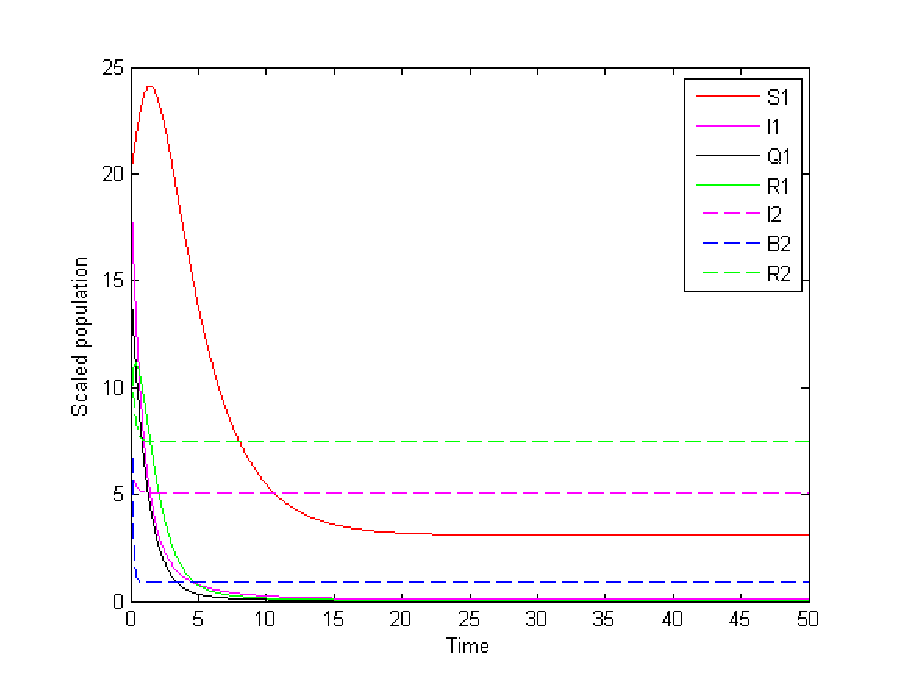
\includegraphics[width=15cm,height=10cm]{13-DR6}}
\caption{Graph between node density and time for set C with initial population (20, 20, 15, 10, 10, 20, 10)}
\label{fig:13-DR6}
\end{figure}
\begin{figure}
\centerline{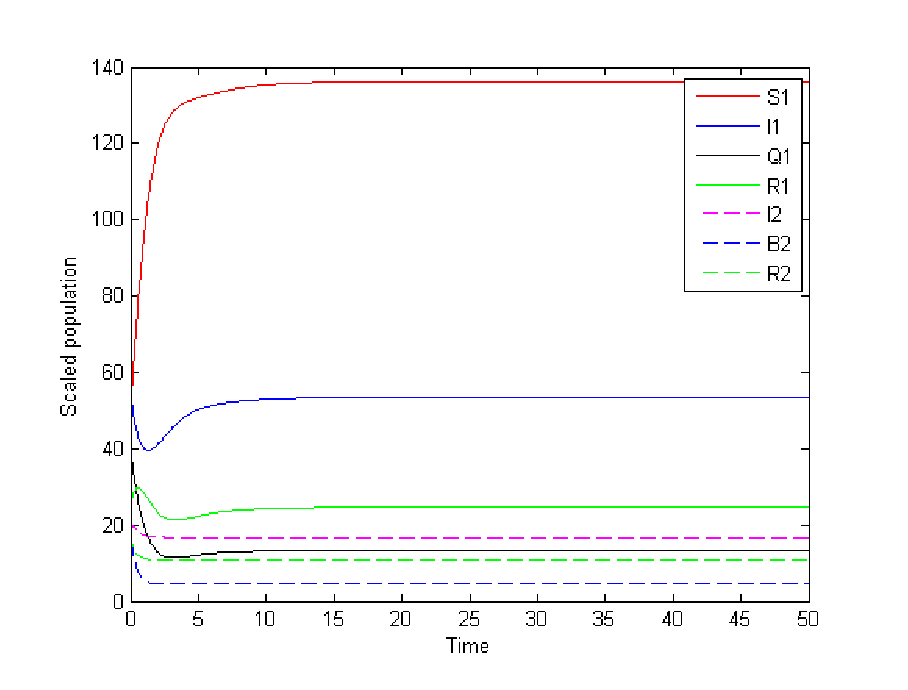
\includegraphics[width=15cm,height=10cm]{13-DR5}}
\caption{Graph between node density and time for set D with initial population (50, 55, 40, 25, 10, 20, 25)}
\label{fig:13-DR5}
\end{figure}

The graph shown in figure \ref{fig:13-DR2} is plotted according to parameter set A with initial population (0.4, 0.02, 0.1, 0.1, 0.25, 0.25 and 0.25).
It can be seen that node density of $S_1$, $I_2$, $B_2$ and $R_2$ classes at steady state are greater than zero, and $E_1$ is the possible steady state.
It can be seen from the table that $R_{01}$ \textless 1 and $R_{02}$ \textless 1, hence it can be concluded from the figure\ref{fig:13-DR2}
that $E_1$ is the stable steady state, i.e., malicious code free equilibrium is stable.
\par The graph shown in figure \ref{fig:13-DR3} is plotted according to parameter set A with initial population (0.30, 0.30, 0.11, 0.25, 0.50, 0.20 and 0.25).
Similarly, it can be observed that $E_1$ is the feasible steady state, i.e., malicious code free equilibrium is stable.
\par The graph shown in figure \ref{fig:13-DR4} is plotted according to parameter set B with initial population (0.2, 0.01, 0.3, 0.4, 0.4, 0.4 and  0.2).
In the figure \ref{fig:13-DR4} node density of all classes at steady state are greater than zero and $E_1$ and $E_2$ are possible feasible states.
Since $R_{01}$$>$1, it can be observed from the figure \ref{fig:13-DR4} that $E_2$ is the stable steady state, i.e., malicious codes will be present in long run.
\par The graph shown in figure \ref{fig:13-DR8} is plotted according to parameter set B with initial population (0.2, 0.01, 0.03, 0.5, 0.4, 0.8 and 0.2).
Similarly, it can be concluded that $E_2$ is the feasible steady states, i.e., malicious objects will be present in long run.
\par The graph shown in figure \ref{fig:13-DR6} is plotted according to parameter set C with initial population (20, 20, 15, 10, 10, 20 and 10).
It can be seen that the density of $\tilde S_1$, $\tilde I_2$, $\tilde B_2$ and $\tilde R_2$
classes at steady state node are greater than zero, and $E_1$ is possible feasible state. Since $\tilde R_0$ \textless 1, it can be observed from the figure\ref{fig:13-DR6}
that $E_1$ is the stable steady state, i.e., malicious code free equilibrium is stable.
\par The graph shown in figure \ref{fig:13-DR5} is plotted according to parameter set D with initial population (50, 55, 40, 25, 10, 20 and 25).
In the figure \ref{fig:13-DR5} at steady state node density of all classes are greater than zero.
In this figure at steady state node density of all classes are greater than zero and both states, $E_1$ and $E_2$, are feasible.
Since $\tilde R_0$$>$1, it can be assured that $E_2$ is the stable steady state, i.e., Malicious codes will be present in long run.
\subsection{Special Cases}
In this subsection, we will study the dynamics of system,
when the internal security, i.e., both anti-virus coefficient, $m_1$ and firewall coefficient, $m_2$ are zero.
\begin{figure}
\centerline{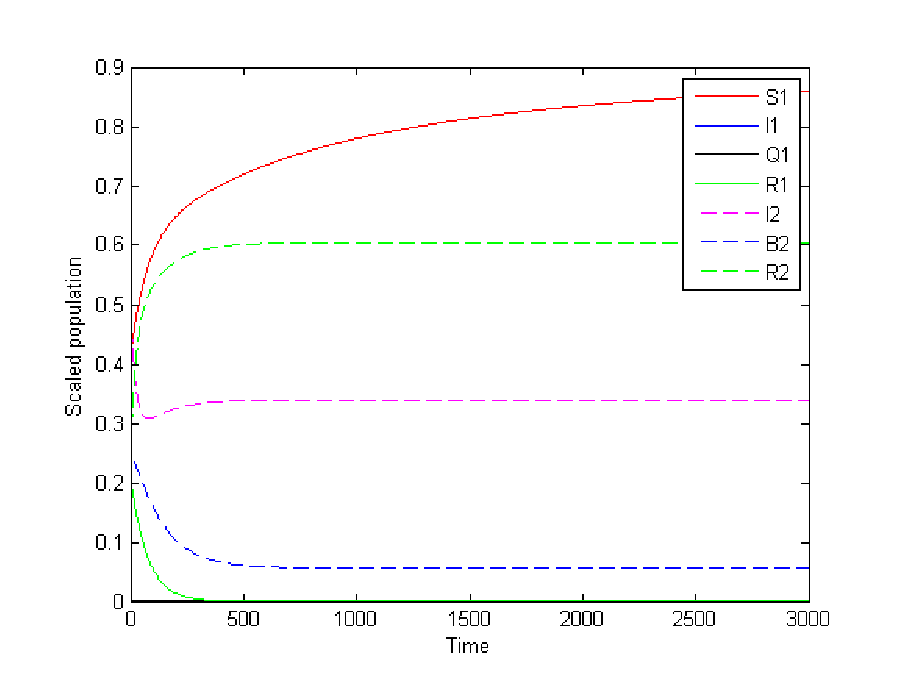
\includegraphics[width=15cm,height=10cm]{13-DR10}}
\caption{Graph between Node Density and Time for set A with initial population (0.4  0.02  0.02  0.2  0.50  0.25  0.25)}
\label{fig:13-DR10}
\end{figure}
\begin{figure}
\centerline{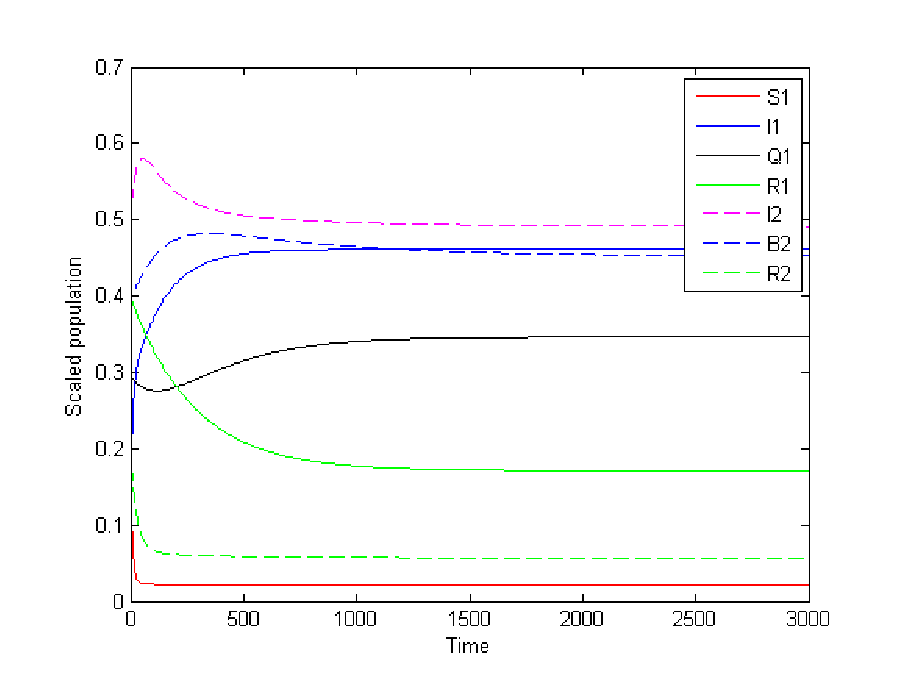
\includegraphics[width=15cm,height=10cm]{13-DR15}}
\caption{Graph between Node Density and Time for set B with initial population (0.2  0.1  0.3  0.4  0.5  0.4  0.2)}
\label{fig:13-DR15}
\end{figure}
\begin{figure}
\centerline{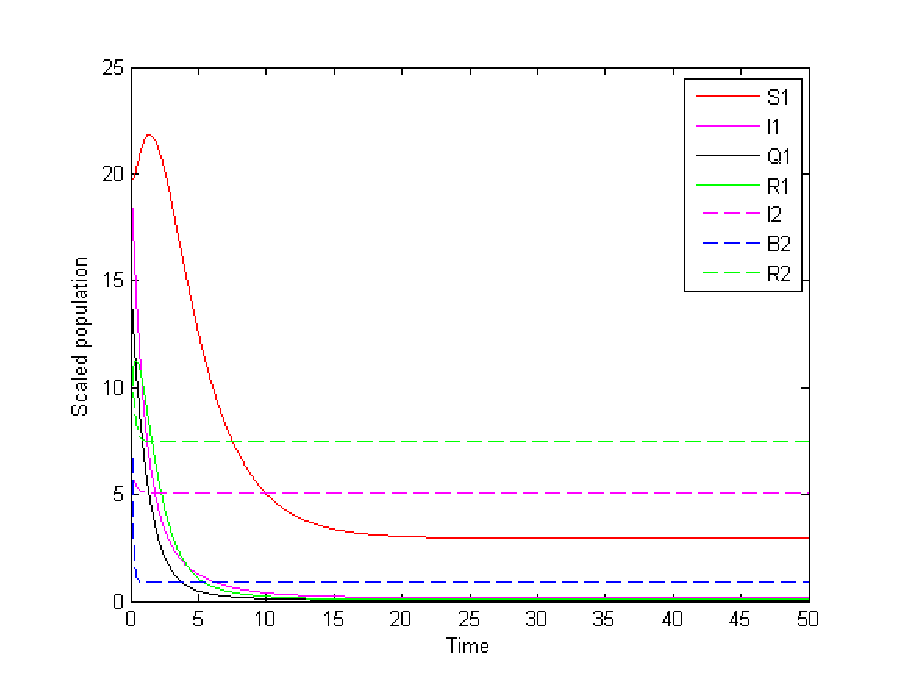
\includegraphics[width=15cm,height=10cm]{13-DR16}}
\caption{Graph between Node Density and Time for set C with initial population (20 20 15 10 10 20 10)}
\label{fig:13-DR16}
\end{figure}
\begin{figure}
\centerline{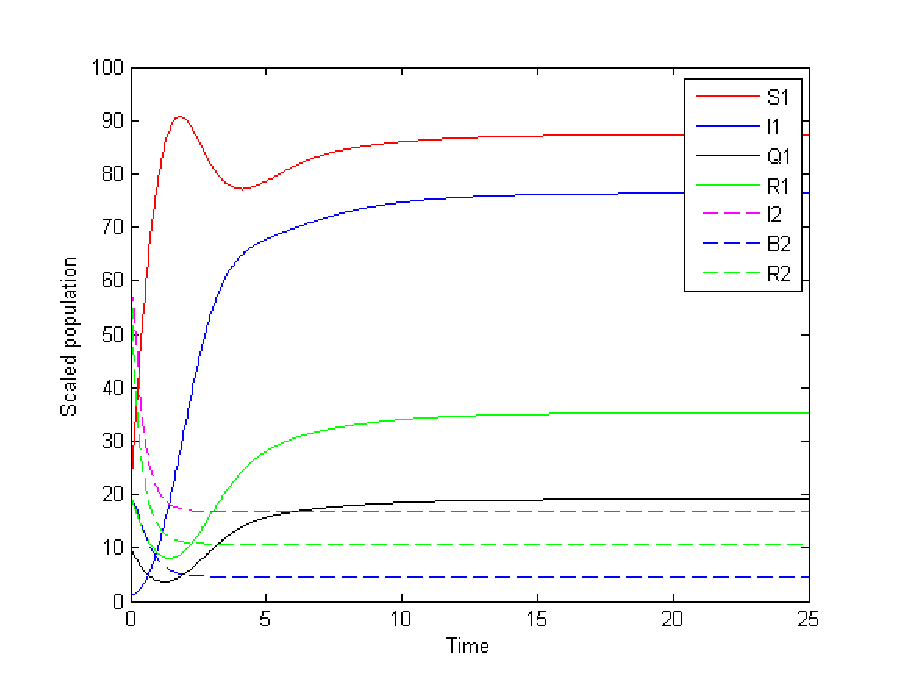
\includegraphics[width=15cm,height=10cm]{13-DR7}}
\caption{Graph between Node Density and Time for set D with initial population (20 1 10 20 50 20 75)}
\label{fig:13-DR7}
\end{figure}
\par Figures  \ref{fig:13-DR10},  \ref{fig:13-DR15},  \ref{fig:13-DR16} and
\ref{fig:13-DR7} are plotted with same parameters that are given in Set A, B, C
and D respectively in the table \ref{table:feas} except the controlling parameters. However, it can be seen
that without controlling factors, the scaled population of Susceptible nodes
 deviates and decreases with respect to time and similarly, the infected population grows.
\par From  all the graphs, it is observed that the natures of graphs are
similar to the earlier graphs with respect to time, for all the values of
basic reproduction number. So, it can
 be concluded that the qualitative features of the model don't change
 due to change in controlling coefficients.
\clearpage
\section{Estimation of media coverage factor (firewall security coefficient)}
Firewall is the computer network security system that observes and controls
 the entering and outgoing traffic of the network based on predetermined security patterns
  and policies. The firewall critically makes a barrier between a trusted as well as
  secure internal computer network and malicious users that are assumed not
   to be secure or trusted.
\subsection{ Order of Rule Enforcement}
The traffic through the particular network connection is examined by the firewall. The
 firewall monitors every connection and then the rules for various factors,
 i.e., IP Address, Port, Domain name, keywords, etc. are enforced sequentially.
  The firewall observes every connection and compares that link for
  the consistency with service,
data and destination. If the connection is valid, then firewall applies
that particular rule otherwise,
it checks for the next matching rule in its predefined Rule base.
\subsection{Firewall rule priority}
Because firewall rules that possess possible conflicts can be determined, it is important to figure out
 the sequence in which the rules are executed.
\subsection{Authenticated bypass}
Authenticated bypass is the rule which enables user to create rules for Firewall with Advanced Security
that blocks incoming traffic unless it is from a specified trusted computer or user.
These rules should allow the propagation of matched network traffic otherwise it would not be given access. A separate security rule for establishment of connection
would be used for the network traffic authentication. These patterns and policies
are used to allow access to any computer to an authorized troubleshooting devices and
network administrators \cite{edtr15}.
\subsection{Block connection}
These rules restrict all matched incoming network traffic if it is found suspicious according to these rules.
\clearpage
\subsection{Allow connection}
These defined rules allow matched incoming network traffic nevertheless the informational data is nontrust-able.
 Because the general criterion is to avoid and stop malicious incoming network traffic, there should be
 a rule for allowance defined to help any network service or program that must accept the incoming traffic.
The coefficient of firewall security, '$m$' should be dependent upon the types of files(data) under
consideration, defined rules of firewall security in firewall rule base and the reliability
and efficiency of the software(firewall) \cite{edtr15}. A way of measuring the value m of firewall
security is defined as:
\begin{equation} m = - log_2 (a+b-ab) \end{equation}
\par Where '$b$' measures the response of the data to the determined security rules. For the
analysis purpose, some rules can be added certainly by observing the nature of attacker population. Firewall will check those rules
firewall rule base when the files or data will be received in targeted class. If these data respond correctly to all rules, then $b$=0 and if not,
then $b$=1 and it is expected that the rate of malware propagation
can be drawn away by proportion '$a$', when each received files tolerate the predetermined security rules \cite{edtr15}.
\clearpage
From figures \ref{fig:13-DR13} to \ref{fig:13-DR12}, it can be seen that for the both case of reproduction number, the fraction of infected population decreases with respect to time as the values of firewall and anti-virus  coefficients increase.
\par The work of  firewall is just to minimize damage caused by spyware by blocking unauthorized and malicious party access, while antivirus is used for the prevention, detection, and removal of malicious software from the system. So, the effect of antivirus and firewall can be seen by the figures \ref{fig:13-DR13} to \ref{fig:13-DR12}.

\begin{figure}[h]
\centerline{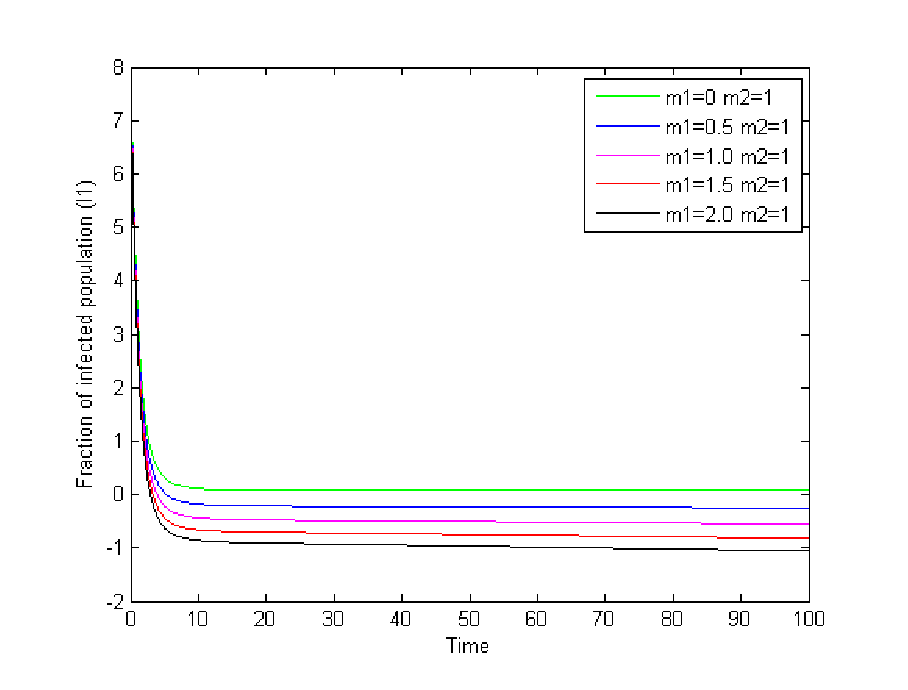
\includegraphics[width=15cm,height=10cm]{13-DR13}}
\caption{Effect of $m_1$ (antivirus coefficient) on $ \tilde I_1$ when $\tilde R_0 < 1$}
\label{fig:13-DR13}
\end{figure}
\begin{figure}[h]
\centerline{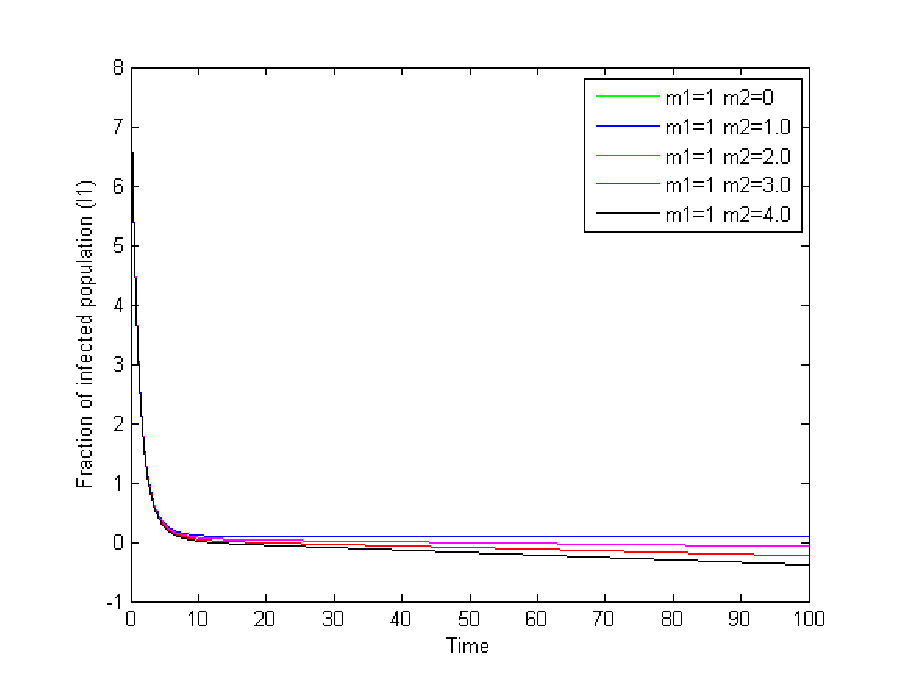
\includegraphics[width=15cm,height=10cm]{13-DR11}}
\caption{Effect of $m_2$ (firewall coefficient) on $ \tilde I_1$ when $\tilde R_0 < 1$}
\label{fig:13-DR11}
\end{figure}
\begin{figure}[h]
\centerline{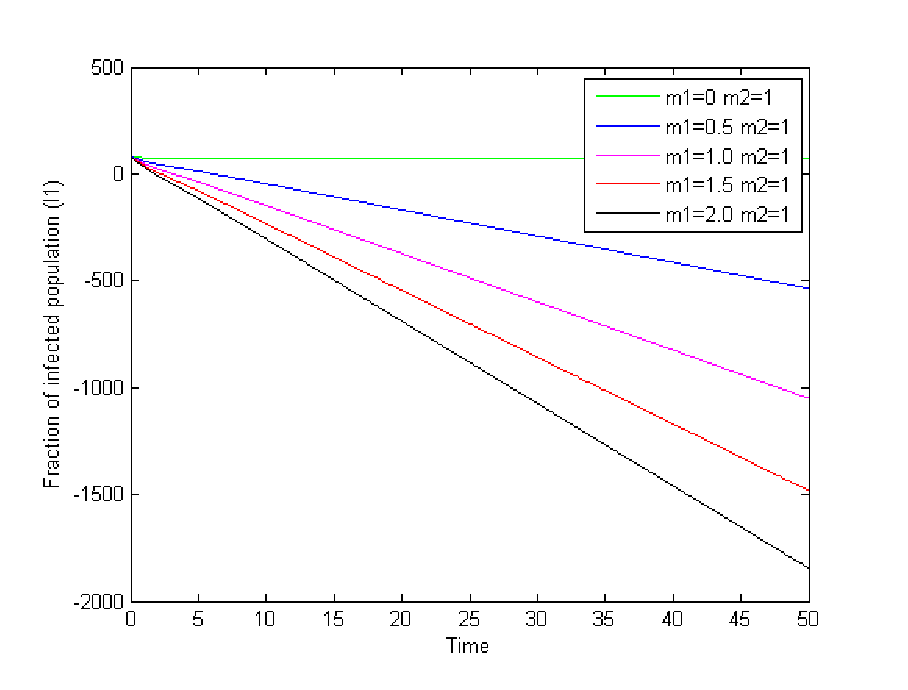
\includegraphics[width=15cm,height=10cm]{13-DR14}}
\caption{Effect of $m_1$ (antivirus coefficient) on $ \tilde I_1$ when $\tilde R_0 > 1$}
\label{fig:13-DR14}
\end{figure}
\begin{figure}[h]
\centerline{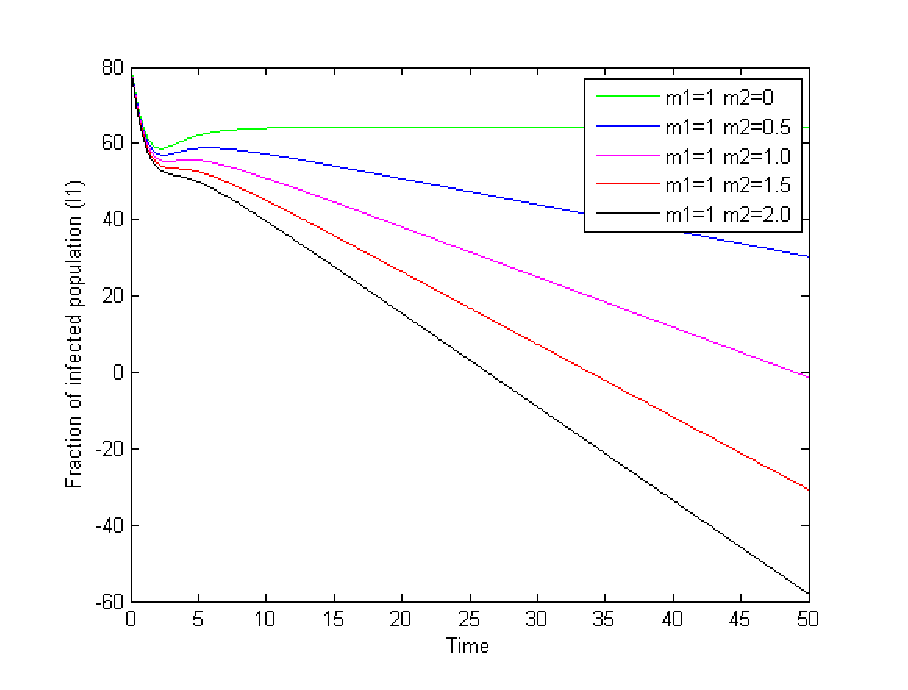
\includegraphics[width=15cm,height=10cm]{13-DR12}}
\caption{Effect of $m_2$ (firewall coefficient) on $ \tilde I_1$ when $\tilde R_0 > 1$}
\label{fig:13-DR12}
\end{figure}
\clearpage
\section{Sensitivity Analysis}
In this step, normalized forward sensitivity index is used for the sensitivity analysis concerning
basic reproduction number. The relative change in a state variable with respect to a
bit change in the system parameter is quantified using sensitivity indices. The ratio of the
relative variation (or change) in the variable to the relative change in the particular system
parameter is defined as the distributed forward sensitivity index of the variable to that particular parameter.
The sensitivity index can also be derived using partial derivatives \cite{edtr14}. Let $p$ is a
 parameter and $u$ is the function of $p$, a little change $\delta$ $p$ to the parameter $p$ and the corresponding change in $u$ as $\delta$ $u$:
\begin{equation} \delta u = u(p + \delta p) - u(p) =[ u(p + \delta p) - u(p)].\frac{\delta p}{\delta p} \equiv \delta p \frac{\partial u}{\partial p}. \end{equation}
The distributed forward sensitivity index for a variable, $u$, which depends on a parameter, $p$, can be defined as:
\begin{equation} \Upsilon_p^u =\frac{\partial u}{\partial p}\times \frac{p}{u} .\end{equation}
\par The prediction and measurement of more sensitive parameter has to be done thoughtfully, because a little change in the parameter will result in relatively huge quantitative change. However, estimation of less sensitive parameter should not require as much practice, since a small change in the parameter, will not lead to huge variation in the quantity.
\par The analytical expressions for sensitivity index of $R_{0}$, with respect to each parameter, are derived. The normalized sensitivity indices for parameters are retrieved as given by the following tables.\\
The sensitivity indices of the basic reproduction numbers $R_{01}$ and $R_{02}$ for all the sets using different parameters are as follows:
\clearpage
1. Distributed sensitivity indices for (non-dimensional) parameters set with respect to $R_{01}$ is shown in table 3.2.
\begin{table}[h]
\label{table:sens}
\begin{tabular}{|p{3 cm}|p{4 cm}|p{3 cm}|p{3 cm}|}
\hline
\bf Parameters ($y_j$) & \bf Sensitivity $ \Upsilon_{y_j}^{R_{01}} $&\bf $ \Upsilon_{y_j}^{R_{01}} $ Set 1&\bf $ \Upsilon_{y_j}^{R_{01}} $ Set 2 \\
\hline
b &0&0&0\\
$d_1$ &0&0&0\\
$\beta_1$ &$\frac{\beta_1}{\beta_1 +1}$&0.000999&0.0099\\
$\beta_2$ &0&0&0\\
$\mu$ &$-\frac{\mu}{d_2+\mu+\eta+1}$&-0.002&-0.00298\\
$\lambda_0$ &0&0&0\\
$d_4$ &0&0&0\\
$b_1$ &0&0&0\\
$d_3$ &0&0&0\\
$\eta$ &$-\frac{\eta}{d_2+\mu+\eta+1}$&-0.0028&-0.000397\\
$\eta_1$ &0&0&0\\
$\alpha$ &0&0&0\\
$d_2$ &$-\frac{d_2}{d_2+\mu+\eta+1}$&-0.28&-0.00397\\
$\gamma$ &0&0&0\\
$\delta$&0&0&0\\
$\theta$ &0&0&0\\
\hline
\end{tabular}
\caption {Distributed sensitivity indices for (non-dimensional) parameters set concerning $R_{01}$ }
\end{table}
\par
It is observed that $d_2$, $\beta_1$, $\mu$ and $\eta$ are moderately
sensitive and rest are independent of $R_{01}$ . For example, $ \Upsilon_{d_2}^{R_{01}} $
for set 1 = -0.28, hence, increasing (decreasing) $d_2$ by 1 \% will decrease (increase) $R_{01}$ by
0.28\%.
\clearpage
 2. Distributed sensitivity indices for parameters (non-dimensional) set with respect to $R_{02}$ is shown in table 3.3.
\begin{table}[h]
\label{table:senst}
\begin{tabular}{|p{3 cm}|p{4 cm}|p{3 cm}|p{3 cm}|}
\hline
\bf Parameters ($y_j$) & \bf Sensitivity $ \Upsilon_{y_j}^{R_{02}} $&\bf $ \Upsilon_{y_j}^{R_{02}} $ Set 1&\bf $ \Upsilon_{y_j}^{R_{02}} $ Set 2 \\
\hline
b &0&0&0\\
$d_1$ &0&0&0\\
$\beta_1$ &0&0&0\\
$\beta_2$ &0&0&0\\
$\mu$ &0&0&0\\
$\lambda_0$ &$-\frac{\lambda_0}{1+d_2+\lambda_0}$&-0.287&-0.00398\\
$d_4$ &0&0&0\\
$b_1$ &0&0&0\\
$d_3$ &0&0&0\\
$\eta$ &0&0&0\\
$\eta_1$ &0&0&0\\
$\alpha$ &0&0&0\\
$d_2$ &$-\frac{d_2}{1+d_2+\lambda_0}$&-0.0057&-0.000796\\
$\gamma$ &0&0&0\\
$\delta$&0&0&0\\
$\theta$ &0&0&0\\
\hline
\end{tabular}
\caption {Distributed sensitivity indices for (non-dimensional) parameters set concerning $R_{02}$ }
\end{table}

\par It is observed that $\lambda$ and $d_2$ are moderately
sensitive, and rest are independent of $R_{02}$ .
\clearpage
3. Distributed sensitivity indices for (dimensional) parameters set with respect to $\tilde R_0$ is shown in the table 3.4.
\begin{table}[h]
\label{table:sensi}
\begin{tabular}{|p{3 cm}|p{4 cm}|p{3 cm}|p{3 cm}|}
\hline
\bf Parameters ($y_j$) & \bf Sensitivity $ \Upsilon_{y_j}^{\tilde R_0} $&\bf $ \Upsilon_{y_j}^{\tilde R_0} $ Set 1&\bf $ \Upsilon_{y_j}^{\tilde R_0} $ Set 2\\
\hline
b &0&0&0\\
$d_1$ &0&0&0\\
$\tilde \beta_1$ &1&1&1\\
$\tilde \beta_2$ &0&0&0\\
$\tilde\mu$ &$-\frac{\tilde \mu}{\tilde d_2+\tilde \mu+\tilde\eta}$&-0.27&-0.27\\
$\tilde\lambda_0$ &$0$&0&0\\
$\tilde d_4$ &0&0&0\\
$\tilde b_1$ &0&0&0\\
$\tilde d_3$ &0&0&0\\
$\tilde\eta$ &$-\frac{\tilde \eta}{\tilde d_2+\tilde \mu+\tilde\eta}$&-0.36&-0.36\\
$\tilde\eta_1$ &0&0&0\\
$\tilde\alpha$ &0&0&0\\
$\tilde d_2$ &$-\frac{\tilde d_2}{\tilde d_2+\tilde \mu+\tilde\eta}$&-0.36&-0.36\\
$\tilde \gamma$ &0&0&0\\
$\tilde \delta$&0&0&0\\
$\tilde \theta$ &0&0&0\\
\hline
\end{tabular}
\caption {Distributed sensitivity indices for (dimensional) parameters set concerning $\tilde R_0$ }
\end{table}
\par From table, It is observed that $\tilde d_2$ and $\tilde \eta$, $\tilde \mu$ are moderately
sensitive and rest are independent of $\tilde R_0$. For example, $ \Upsilon_{\tilde d_2}^{\tilde R_0}$
for set 1 = -0.36, hence, increasing (decreasing) $\tilde d_2$ by 1\% will decrease (increase) $\tilde R_0$ by
0.36\%.
\par In the next chapter, the conclusion and the future scope are discussed. 